\begin{flushleft}
	\section{\textcolor{cyan}{Circuits électriques : Schéma, câblage et branchement :}}
	
	\subsection{\textcolor{green}{Interfaçage écran OLED SSD1306 avec Esp8266}}
	\subsubsection{\textcolor{blue}{Câblage de l'écran OLED SSD1306 sur l'Esp8266 :}}

		\begin{figure}[h]
			\centering
			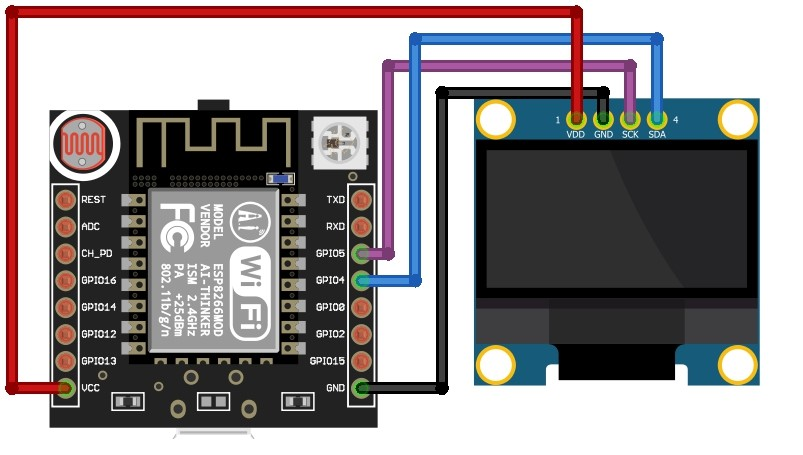
\includegraphics{chapitres/images/esp8266-oled1306.jpg}
			\caption{Câblage de l'écran OLED SSD1306 sur l'Esp8266}
			\label{fig:labelname}
		\end{figure}
	
	\begin{lstlisting}[style=CStyle]
		#include <Wire.h> // Include the Wire.h library to communicate in I2C
		#include <Adafruit_GFX.h> // Include the Adafruit_GFX.h library for graphics support
		#include <Adafruit_SSD1306.h> // Include Adafruit_SSD1306.h library for OLED display
		
		#define SCREEN_WIDTH 128 // OLED screen width in pixels
		#define SCREEN_HEIGHT 64 // Height of the OLED screen in pixels
		
		// OLED screen initialization
		Adafruit_SSD1306 display(SCREEN_WIDTH, SCREEN_HEIGHT, &Wire, -1);
		
		void setup() {
			// Initializing serial communication for debugging
			Serial.begin(9600);
			
			// OLED display initialization with I2C address 0x3C (default for SSD1306 display)
			if(!display.begin(SSD1306_SWITCHCAPVCC, 0x3C)) {
				Serial.println(F("Error: OLED screen not detected"));
				while (true);
			}
			
			// Clear OLED screen
			display.clearDisplay();
			display.display();
		}
		
		void loop() {
			// Display the message "Hello!" on the OLED display
			display.setTextSize(2);
			display.setTextColor(WHITE);
			display.setCursor(0, 0);
			display.println("Bonjour !");
			display.display();
			
			// Wait 2 seconds before trying again
			delay(2000);
		}
		
	\end{lstlisting}
	
	
	
	\subsection{\textcolor{green}{Interfaçage de l’oxymètre de pouls MAX30102 et du capteur de fréquence cardiaque avec Esp8266}}
	
	
	\subsubsection{\textcolor{blue}{Câblage d’un module MAX30102 sur l'Esp8266 :}}
	\begin{figure}[h]
		\begin{minipage}{0.6\textwidth}
			\underline{NIV} est la broche d’alimentation. Vous pouvez le connecter à une sortie 3.3V ou 5V de votre Arduino.
			
			\underline{SCL} est la broche de l’horloge I2C, connectez-vous à la ligne d’horloge I2C de votre Arduino.
			
			\underline{SDA} est la broche de données I2C, connectez-vous à la ligne de données I2C de votre Arduino.
			
			\underline{INT} Le MAX30102 peut être programmé pour générer une interruption pour chaque impulsion. Cette ligne est à vidange ouverte, elle est donc tirée HAUT par la résistance embarquée. Lorsqu’une interruption se produit, la broche INT devient LOW et reste LOW jusqu’à ce que l’interruption soit effacée.
			
			\underline{IRD} Le MAX30102 intègre un pilote LED pour piloter les impulsions LED pour les mesures SpO2 et HR. Utilisez-le si vous souhaitez piloter vous-même la LED IR, sinon laissez-la déconnectée.
			
			\underline{RD} La broche est similaire à la broche IRD, mais est utilisée pour piloter la LED rouge. Si vous ne voulez pas piloter la LED rouge vous-même, laissez-la déconnectée.
			
			\underline{GND} est le sol. image.
		\end{minipage}
		\begin{minipage}{0.4\textwidth}
			\centering
			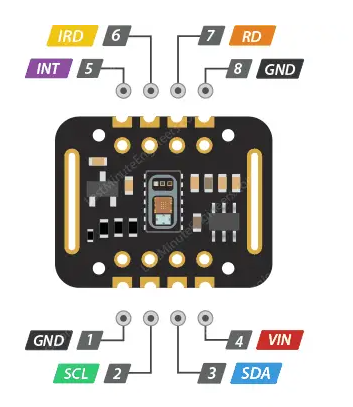
\includegraphics[width=\textwidth]{chapitres/images/Capteur8.PNG}
			\caption{Brochage du module MAX30102}
			\label{fig:votre_image}
		\end{minipage}
	\end{figure}

		\begin{figure}[h]
			\centering
			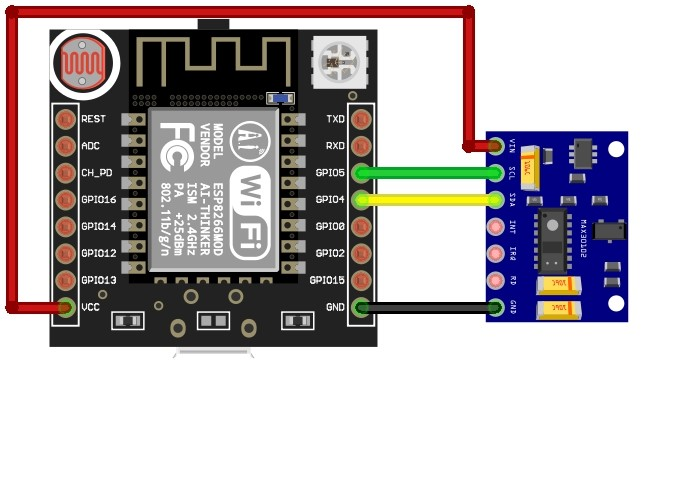
\includegraphics{chapitres/images/MAX30102-with-ESP8266.jpg}
			\caption{Câblage d’un module MAX30102 sur l'Esp8266}
			\label{fig:labelname}
		\end{figure}
\newpage
	\subsubsection{\textcolor{blue}{Lecture du température}}
	\begin{lstlisting}[style=CStyle]
		#include <Wire.h>
		
		#include "MAX30105.h"
		MAX30105 particleSensor;
		
		void setup() {
			Serial.begin(9600);
			Serial.println("Initializing...");
			
			// Initialize sensor
			if (particleSensor.begin(Wire, I2C_SPEED_FAST) == false) { //Use default I2C port, 400kHz speed
				Serial.println("MAX30102 was not found. Please check wiring/power. ");
				while (1);
			}
			
			//The LEDs are very low power and won't affect the temp reading much but
			//you may want to turn off the LEDs to avoid any local heating
			particleSensor.setup(0); //Configure sensor. Turn off LEDs
			
			particleSensor.enableDIETEMPRDY(); //Enable the temp ready interrupt. This is required.
		}
		
		void loop() {
			float temperature = particleSensor.readTemperature();
			
			Serial.print("temperatureC=");
			Serial.print(temperature, 4);
			
			float temperatureF = particleSensor.readTemperatureF();
			
			Serial.print(" temperatureF=");
			Serial.print(temperatureF, 4);
			
			Serial.println();
		}
	\end{lstlisting}
	
	
	
	\subsubsection{\textcolor{blue}{Mesure de la fréquence cardiaque (BPM)}}
	\begin{lstlisting}[style=CStyle]
		#include <Wire.h>
		#include "MAX30105.h"
		#include "heartRate.h"
		
		MAX30105 particleSensor;
		
		const byte RATE_SIZE = 4; //Increase this for more averaging. 4 is good.
		byte rates[RATE_SIZE]; //Array of heart rates
		byte rateSpot = 0;
		long lastBeat = 0; //Time at which the last beat occurred
		
		float beatsPerMinute;
		int beatAvg;
		
		void setup() {
			Serial.begin(115200);
			Serial.println("Initializing...");
			
			// Initialize sensor
			if (!particleSensor.begin(Wire, I2C_SPEED_FAST)) {
				Serial.println("MAX30102 was not found. Please check wiring/power. ");
				while (1);
			}
			Serial.println("Place your index finger on the sensor with steady pressure.");
			
			particleSensor.setup(); //Configure sensor with default settings
			particleSensor.setPulseAmplitudeRed(0x0A); //Turn Red LED to low to indicate sensor is running
			particleSensor.setPulseAmplitudeGreen(0); //Turn off Green LED
		}
		
		void loop() {
			long irValue = particleSensor.getIR();
			
			if (checkForBeat(irValue) == true) {
				//We sensed a beat!
				long delta = millis() - lastBeat;
				lastBeat = millis();
				
				beatsPerMinute = 60 / (delta / 1000.0);
				
				if (beatsPerMinute < 255 && beatsPerMinute > 20) {
					rates[rateSpot++] = (byte)beatsPerMinute; //Store this reading in the array
					rateSpot %= RATE_SIZE; //Wrap variable
					
					//Take average of readings
					beatAvg = 0;
					for (byte x = 0 ; x < RATE_SIZE ; x++)
					beatAvg += rates[x];
					beatAvg /= RATE_SIZE;
				}
			}
			
			Serial.print("IR=");
			Serial.print(irValue);
			Serial.print(", BPM=");
			Serial.print(beatsPerMinute);
			Serial.print(", Avg BPM=");
			Serial.print(beatAvg);
			
			if (irValue < 50000)
			Serial.print(" No finger?");
			
			Serial.println();
		}
	\end{lstlisting}
	\subsubsection{\textcolor{blue}{Mesure de la saturation en oxygène (SpO2)}}
	\begin{lstlisting}[style=CStyle]
		#include <Wire.h>
		#include "MAX30105.h"
		#include "spo2_algorithm.h"
		
		MAX30105 particleSensor;
		
		#define MAX_BRIGHTNESS 255
		
		#if defined(__AVR_ATmega328P__) || defined(__AVR_ATmega168__)
		//Arduino Uno doesn't have enough SRAM to store 100 samples of IR led data and red led data in 32-bit format
		//To solve this problem, 16-bit MSB of the sampled data will be truncated. Samples become 16-bit data.
		uint16_t irBuffer[100]; //infrared LED sensor data
		uint16_t redBuffer[100];  //red LED sensor data
		#else
		uint32_t irBuffer[100]; //infrared LED sensor data
		uint32_t redBuffer[100];  //red LED sensor data
		#endif
		
		int32_t bufferLength; //data length
		int32_t spo2; //SPO2 value
		int8_t validSPO2; //indicator to show if the SPO2 calculation is valid
		int32_t heartRate; //heart rate value
		int8_t validHeartRate; //indicator to show if the heart rate calculation is valid
		
		byte pulseLED = 11; //Must be on PWM pin
		byte readLED = 13; //Blinks with each data read
		
		void setup()
		{
			Serial.begin(115200); // initialize serial communication at 115200 bits per second:
			
			pinMode(pulseLED, OUTPUT);
			pinMode(readLED, OUTPUT);
			
			// Initialize sensor
			if (!particleSensor.begin(Wire, I2C_SPEED_FAST)) //Use default I2C port, 400kHz speed
			{
				Serial.println(F("MAX30105 was not found. Please check wiring/power."));
				while (1);
			}
			
			Serial.println(F("Attach sensor to finger with rubber band. Press any key to start conversion"));
			while (Serial.available() == 0) ; //wait until user presses a key
			Serial.read();
			
			byte ledBrightness = 60; //Options: 0=Off to 255=50mA
			byte sampleAverage = 4; //Options: 1, 2, 4, 8, 16, 32
			byte ledMode = 2; //Options: 1 = Red only, 2 = Red + IR, 3 = Red + IR + Green
			byte sampleRate = 100; //Options: 50, 100, 200, 400, 800, 1000, 1600, 3200
			int pulseWidth = 411; //Options: 69, 118, 215, 411
			int adcRange = 4096; //Options: 2048, 4096, 8192, 16384
			
			particleSensor.setup(ledBrightness, sampleAverage, ledMode, sampleRate, pulseWidth, adcRange); //Configure sensor with these settings
		}
		
		void loop()
		{
			bufferLength = 100; //buffer length of 100 stores 4 seconds of samples running at 25sps
			
			//read the first 100 samples, and determine the signal range
			for (byte i = 0 ; i < bufferLength ; i++)
			{
				while (particleSensor.available() == false) //do we have new data?
				particleSensor.check(); //Check the sensor for new data
				
				redBuffer[i] = particleSensor.getRed();
				irBuffer[i] = particleSensor.getIR();
				particleSensor.nextSample(); //We're finished with this sample so move to next sample
				
				Serial.print(F("red="));
				Serial.print(redBuffer[i], DEC);
				Serial.print(F(", ir="));
				Serial.println(irBuffer[i], DEC);
			}
			
			//calculate heart rate and SpO2 after first 100 samples (first 4 seconds of samples)
			maxim_heart_rate_and_oxygen_saturation(irBuffer, bufferLength, redBuffer, &spo2, &validSPO2, &heartRate, &validHeartRate);
			
			//Continuously taking samples from MAX30102.  Heart rate and SpO2 are calculated every 1 second
			while (1)
			{
				//dumping the first 25 sets of samples in the memory and shift the last 75 sets of samples to the top
				for (byte i = 25; i < 100; i++)
				{
					redBuffer[i - 25] = redBuffer[i];
					irBuffer[i - 25] = irBuffer[i];
				}
				
				//take 25 sets of samples before calculating the heart rate.
				for (byte i = 75; i < 100; i++)
				{
					while (particleSensor.available() == false) //do we have new data?
					particleSensor.check(); //Check the sensor for new data
					
					digitalWrite(readLED, !digitalRead(readLED)); //Blink onboard LED with every data read
					
					redBuffer[i] = particleSensor.getRed();
					irBuffer[i] = particleSensor.getIR();
					particleSensor.nextSample(); //We're finished with this sample so move to next sample
					
					//send samples and calculation result to terminal program through UART
					Serial.print(F("red="));
					Serial.print(redBuffer[i], DEC);
					Serial.print(F(", ir="));
					Serial.print(irBuffer[i], DEC);
					
					Serial.print(F(", HR="));
					Serial.print(heartRate, DEC);
					
					Serial.print(F(", HRvalid="));
					Serial.print(validHeartRate, DEC);
					
					Serial.print(F(", SPO2="));
					Serial.print(spo2, DEC);
					
					Serial.print(F(", SPO2Valid="));
					Serial.println(validSPO2, DEC);
				}
				
				//After gathering 25 new samples recalculate HR and SP02
				maxim_heart_rate_and_oxygen_saturation(irBuffer, bufferLength, redBuffer, &spo2, &validSPO2, &heartRate, &validHeartRate);
			}
		}
	\end{lstlisting}
	\newpage
\end{flushleft}